% answers.tex —— 2009 年·全国大纲卷Ⅰ·文科 · 参考答案与详细解析片段
% 由 tools/generate_projects.py 依来源总账自 2009/2009_数学真题_全国1文_试题.md + 2009/2009_数学真题_全国1文_解析正文.md + 2009/2009_数学真题_全国1文_答案要点.md 生成，勿手改（改源 MD 后重跑）


\begin{gktip}
固定源 PDF 为印刷页码 509–510 的两页题面，不附答案。以下解析均依据固定源独立复算；第 20、23 题图形在 LaTeX 工程中以 TikZ/PGFPlots 矢量源重绘。
\end{gktip}

\begin{answer}
\gksolhead{1}{}

\textbf{题目}：

$\sin585^\circ$ 的值为\mbox{（　　）}

（A）$-\dfrac{\sqrt2}{2}$\quad（B）$\dfrac{\sqrt2}{2}$\quad（C）$-\dfrac{\sqrt3}{2}$\quad（D）$\dfrac{\sqrt3}{2}$

\Needspace{4\baselineskip}
\textbf{解析}

$585^\circ=360^\circ+225^\circ$，故 $\sin585^\circ=-\dfrac{\sqrt2}{2}$，选 A。

\gkanswer{答案：A}

\end{answer}
\begin{answer}
\gksolhead{2}{}

\textbf{题目}：

设集合 $A=\{4,5,7,9\}$，$B=\{3,4,7,8,9\}$，全集 $U=A\cup B$，则集合 $\complement_U(A\cap B)$ 中的元素共有\mbox{（　　）}

（A）$3$ 个\quad（B）$4$ 个\quad（C）$5$ 个\quad（D）$6$ 个

\Needspace{4\baselineskip}
\textbf{解析}

$A\cap B=\{4,7,9\}$，$U=\{3,4,5,7,8,9\}$，所以
$\complement_U(A\cap B)=\{3,5,8\}$，选 A。

\gkanswer{答案：A}

\end{answer}
\begin{answer}
\gksolhead{3}{}

\textbf{题目}：

不等式 $\left|\dfrac{x+1}{x-1}\right|<1$ 的解集为\mbox{（　　）}

（A）$\{x\mid0<x<1\}\cup\{x\mid x>1\}$\quad（B）$\{x\mid0<x<1\}$\quad（C）$\{x\mid-1<x<0\}$\quad（D）$\{x\mid x<0\}$

\Needspace{4\baselineskip}
\textbf{解析}

\nopagebreak[4]
\[
\left|\frac{x+1}{x-1}\right|<1
\Longleftrightarrow (x+1)^2<(x-1)^2
\Longleftrightarrow x<0,
\]

故选 D。

\gkanswer{答案：D}

\end{answer}
\begin{answer}
\gksolhead{4}{}

\textbf{题目}：

已知 $\tan\alpha=4$，$\cot\beta=\dfrac13$，则 $\tan(\alpha+\beta)=$\mbox{（　　）}

（A）$\dfrac7{11}$\quad（B）$-\dfrac7{11}$\quad（C）$\dfrac7{13}$\quad（D）$-\dfrac7{13}$

\Needspace{4\baselineskip}
\textbf{解析}

\Needspace{5\baselineskip}
由 $\tan\beta=3$，

\nopagebreak[4]
\[
\tan(\alpha+\beta)=\frac{4+3}{1-4\cdot3}=-\frac7{11},
\]

故选 B。

\gkanswer{答案：B}

\end{answer}
\begin{answer}
\gksolhead{5}{}

\textbf{题目}：

设双曲线 $\dfrac{x^2}{a^2}-\dfrac{y^2}{b^2}=1$（$a>0,b>0$）的渐近线与抛物线 $y=x^2+1$ 相切，则该双曲线的离心率等于\mbox{（　　）}

（A）$\sqrt3$\quad（B）$2$\quad（C）$\sqrt5$\quad（D）$\sqrt6$

\Needspace{4\baselineskip}
\textbf{解析}

渐近线为 $y=\pm\dfrac ba x$。与 $y=x^2+1$ 相切时，
$x^2-\dfrac ba x+1=0$ 有重根，故 $\dfrac ba=2$。于是
$e=\sqrt{1+b^2/a^2}=\sqrt5$，选 C。

\gkanswer{答案：C}

\end{answer}
\begin{answer}
\gksolhead{6}{}

\textbf{题目}：

已知函数 $f(x)$ 的反函数为 $g(x)=1+2\lg x$（$x>0$），则 $f(1)+g(1)=$\mbox{（　　）}

（A）$0$\quad（B）$1$\quad（C）$2$\quad（D）$4$

\Needspace{4\baselineskip}
\textbf{解析}

由 $g(1)=1$ 及反函数关系，$f(1)=1$，所以 $f(1)+g(1)=2$，选 C。

\gkanswer{答案：C}

\end{answer}
\begin{answer}
\gksolhead{7}{}

\textbf{题目}：

甲组有 $5$ 名男同学、$3$ 名女同学；乙组有 $6$ 名男同学、$2$ 名女同学。若从甲、乙两组中各选出 $2$ 名同学，则选出的 $4$ 人中恰有 $1$ 名女同学的不同选法共有\mbox{（　　）}

（A）$150$ 种\quad（B）$180$ 种\quad（C）$300$ 种\quad（D）$345$ 种

\Needspace{4\baselineskip}
\textbf{解析}

\Needspace{5\baselineskip}
恰有一名女同学的选法数为

\nopagebreak[4]
\[
\binom31\binom51\binom62+\binom52\binom21\binom61
=225+120=345,
\]

故选 D。

\gkanswer{答案：D}

\end{answer}
\begin{answer}
\gksolhead{8}{}

\textbf{题目}：

设非零向量 $\boldsymbol a,\boldsymbol b,\boldsymbol c$ 满足 $|\boldsymbol a|=|\boldsymbol b|=|\boldsymbol c|$，$\boldsymbol a+\boldsymbol b=\boldsymbol c$，则 $\langle\boldsymbol a,\boldsymbol b\rangle=$\mbox{（　　）}

（A）$150^\circ$\quad（B）$120^\circ$\quad（C）$60^\circ$\quad（D）$30^\circ$

\Needspace{4\baselineskip}
\textbf{解析}

\Needspace{5\baselineskip}
设三个向量的长度均为 $r$。由 $\boldsymbol a+\boldsymbol b=\boldsymbol c$，

\nopagebreak[4]
\[
r^2=2r^2+2\langle\boldsymbol a,\boldsymbol b\rangle,
\]

得夹角为 $120^\circ$，选 B。

\gkanswer{答案：B}

\end{answer}
\begin{answer}
\gksolhead{9}{}

\textbf{题目}：

已知三棱柱 $ABC-A_1B_1C_1$ 的侧棱与底面边长都相等，$A_1$ 在底面 $ABC$ 上的射影为 $BC$ 的中点，则异面直线 $AB$ 与 $CC_1$ 所成的角的余弦值为\mbox{（　　）}

（A）$\dfrac{\sqrt3}{4}$\quad（B）$\dfrac{\sqrt5}{4}$\quad（C）$\dfrac{\sqrt7}{4}$\quad（D）$\dfrac34$

\Needspace{4\baselineskip}
\textbf{解析}

取底面边长和侧棱长为 $2$。$A_1$ 到 $BC$ 中点的水平距离为
$\sqrt3$，故侧棱的竖直分量为 $1$。计算得
$\overrightarrow{AB}\cdot\overrightarrow{CC_1}=3$，两向量长度均为 $2$，
故余弦为 $\dfrac34$，选 D。

\gkanswer{答案：D}

\end{answer}
\begin{answer}
\gksolhead{10}{}

\textbf{题目}：

如果函数 $y=3\cos(2x+\varphi)$ 的图象关于点 $\left(\dfrac{4\pi}{3},0\right)$ 中心对称，那么 $|\varphi|$ 的最小值为\mbox{（　　）}

（A）$\dfrac\pi6$\quad（B）$\dfrac\pi4$\quad（C）$\dfrac\pi3$\quad（D）$\dfrac\pi2$

\Needspace{4\baselineskip}
\textbf{解析}

中心对称点的纵坐标为 $0$，所以
$\dfrac{8\pi}{3}+\varphi=\dfrac\pi2+k\pi$。模 $\pi$ 取最小绝对值，
$\varphi=-\dfrac\pi6$，故选 A。

\gkanswer{答案：A}

\end{answer}
\begin{answer}
\gksolhead{11}{}

\textbf{题目}：

已知二面角 $\alpha-l-\beta$ 为 $60^\circ$，动点 $P\text{、}Q$ 分别在面 $\alpha\text{、}\beta$ 内，$P$ 到 $\beta$ 的距离为 $\sqrt3$，$Q$ 到 $\alpha$ 的距离为 $2\sqrt3$，则 $P\text{、}Q$ 两点之间距离的最小值为\mbox{（　　）}

（A）$\sqrt2$\quad（B）$2$\quad（C）$2\sqrt3$\quad（D）$4$

\Needspace{4\baselineskip}
\textbf{解析}

在垂直于棱的截面内，$P\text{、}Q$ 到棱的距离分别为
\Needspace{5\baselineskip}
$\sqrt3/\sin60^\circ=2$ 和 $2\sqrt3/\sin60^\circ=4$。故

\nopagebreak[4]
\[
PQ_{\min}=\sqrt{2^2+4^2-2\cdot2\cdot4\cos60^\circ}=2\sqrt3,
\]

选 C。

\gkanswer{答案：C}

\end{answer}
\begin{answer}
\gksolhead{12}{}

\textbf{题目}：

已知椭圆 $C:\dfrac{x^2}{2}+y^2=1$ 的右焦点为 $F$，右准线为 $l$，点 $A\in l$，线段 $AF$ 交 $C$ 于点 $B$。若 $\overrightarrow{FA}=3\overrightarrow{FB}$，则 $|\overrightarrow{AF}|=$\mbox{（　　）}

（A）$\sqrt2$\quad（B）$2$\quad（C）$\sqrt3$\quad（D）$3$

\Needspace{4\baselineskip}
\textbf{解析}

右焦点为 $F=(1,0)$，右准线为 $x=2$。设 $A=(2,t)$，则
$B=F+\dfrac13(A-F)=\left(\dfrac43,\dfrac t3\right)$。代入椭圆方程得
$t^2=1$，所以 $|AF|=\sqrt2$，选 A。

\gkanswer{答案：A}

\end{answer}
\begin{answer}
\gksolhead{13}{}

\textbf{题目}：

已知椭圆 $C:\dfrac{x^2}{2}+y^2=1$ 的右焦点为 $F$，右准线为 $l$，点 $A\in l$，线段 $AF$ 交 $C$ 于点 $B$。若 $\overrightarrow{FA}=3\overrightarrow{FB}$，则 $|\overrightarrow{AF}|=$\mbox{（　　）}

（A）$\sqrt2$\quad（B）$2$\quad（C）$\sqrt3$\quad（D）$3$

\begin{gktip}
\textbf{固定源说明}：固定源 PDF 中第 12、13 题的题干和选项逐字相同，暂按原样保留，待取得同版勘误或其他可靠版本后核对。
\end{gktip}

\Needspace{4\baselineskip}
\textbf{解析}

固定源中的第 13 题与第 12 题逐字相同，按同样计算得 $|AF|=\sqrt2$，
选 A；重复题面已挂源级待核问题。

\gkanswer{答案：A}

\end{answer}
\begin{answer}
\gksolhead{14}{}

\textbf{题目}：

$(x-y)^{10}$ 的展开式中，$x^7y^3$ 的系数与 $x^3y^7$ 的系数之和等于\gkblank{}。

\Needspace{4\baselineskip}
\textbf{解析}

两个系数分别为 $-\binom{10}{3}$ 和 $-\binom{10}{7}$，其和为 $-240$。

\gkanswer{答案：$-240$}

\end{answer}
\begin{answer}
\gksolhead{15}{}

\textbf{题目}：

设等差数列 $\{a_n\}$ 的前 $n$ 项和为 $S_n$，若 $S_9=72$，则 $a_2+a_4+a_9=$\gkblank{}。

\Needspace{4\baselineskip}
\textbf{解析}

$S_9=\dfrac92(a_1+a_9)=72$，故 $a_1+a_9=16$。又
$a_2+a_4+a_9=\dfrac32(a_1+a_9)=24$。

\gkanswer{答案：$24$}

\end{answer}
\begin{answer}
\gksolhead{16}{}

\textbf{题目}：

已知 $OA$ 为球 $O$ 的半径，过 $OA$ 的中点 $M$ 且垂直于 $OA$ 的平面截球面得到圆 $M$。若圆 $M$ 的面积为 $3\pi$，则球 $O$ 的表面积等于\gkblank{}。

\Needspace{4\baselineskip}
\textbf{解析}

设球半径为 $R$。截面圆心到球心的距离为 $R/2$，且截面面积为 $3\pi$，
\Needspace{5\baselineskip}
所以

\nopagebreak[4]
\[
3=R^2-\frac{R^2}{4}=\frac34R^2.
\]

故 $R^2=4$，球面面积为 $16\pi$。

\gkanswer{答案：$16\pi$}

\end{answer}
\begin{answer}
\gksolhead{17}{}

\textbf{题目}：

若直线 $m$ 被两平行线 $l_1:x-y+1=0$ 与 $l_2:x-y+3=0$ 所截得的线段的长为 $2\sqrt2$，则 $m$ 的倾斜角可以是

① $15^\circ$　② $30^\circ$　③ $45^\circ$　④ $60^\circ$　⑤ $75^\circ$

其中正确答案的序号是\gkblank{}。（写出所有正确答案的序号）

\Needspace{4\baselineskip}
\textbf{解析}

两平行线距离为 $\sqrt2$。若 $m$ 与它们的夹角为 $\theta$，则
$\sqrt2/\sin\theta=2\sqrt2$，从而 $\sin\theta=1/2$。
平行线倾斜角为 $45^\circ$，故正确倾斜角为 $15^\circ\text{、}75^\circ$，即
①、⑤。

\gkanswer{答案：①、⑤}

\end{answer}
\begin{answer}
\gksolhead{18}{}

\textbf{题目}：

设等差数列 $\{a_n\}$ 的前 $n$ 项和为 $S_n$，公比是正数的等比数列 $\{b_n\}$ 的前 $n$ 项和为 $T_n$，已知 $a_1=1$，$b_1=3$，$a_3+b_3=17$，$T_3-S_3=12$，求 $\{a_n\}$、$\{b_n\}$ 的通项公式。

\Needspace{4\baselineskip}
\textbf{解析}

\Needspace{5\baselineskip}
设等差公差为 $d$，等比公比为 $q>0$。由已知

\nopagebreak[4]
\[
2d+3q^2=16,\qquad q+q^2-d=4.
\]

\Needspace{5\baselineskip}
消去 $d$ 得 $5q^2+2q-24=0$，故 $q=2$、$d=2$。所以

\nopagebreak[4]
\[
a_n=2n-1,\qquad b_n=3\cdot2^{n-1}.
\]

\gkanswer{答案：$a_n=2n-1,\ b_n=3\cdot2^{n-1}$}

\end{answer}
\begin{answer}
\gksolhead{19}{}

\textbf{题目}：

在 $\triangle ABC$ 中，内角 $A\text{、}B\text{、}C$ 的对边长分别为 $a\text{、}b\text{、}c$，已知 $a^2-c^2=2b$，且 $\sin B=4\cos A\sin C$，求 $b$。

\Needspace{4\baselineskip}
\textbf{解析}

\Needspace{5\baselineskip}
由正弦定理和题设，

\nopagebreak[4]
\[
\frac bc=4\cos A.
\]

\Needspace{5\baselineskip}
余弦定理结合 $a^2-c^2=2b$ 得

\nopagebreak[4]
\[
\cos A=\frac{b^2+c^2-a^2}{2bc}=\frac{b-2}{2c}.
\]

故 $\dfrac bc=\dfrac{2(b-2)}c$，解得 $b=4$。

\gkanswer{答案：$b=4$}

\end{answer}
\begin{answer}
\gksolhead{20}{}

\textbf{题目}：

如图，四棱锥 $S-ABCD$ 中，底面 $ABCD$ 为矩形，$SD\perp$ 底面 $ABCD$，$AD=\sqrt2$，$DC=SD=2$，点 $M$ 在侧棱 $SC$ 上，$\angle ABM=60^\circ$。
\nopagebreak[4]
\begin{center}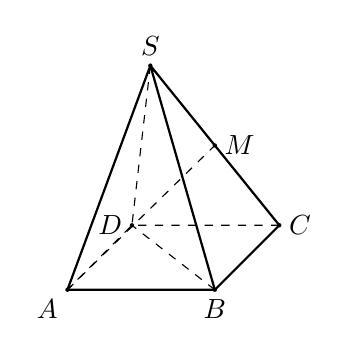
\begin{tikzpicture}[scale=.78,>=stealth]
\coordinate (A) at (0,0); \coordinate (B) at (2.4,0);
\coordinate (C) at (3.45,1.05); \coordinate (D) at (1.05,1.05);
\coordinate (S) at (1.35,3.65); \coordinate (M) at (2.40,2.35);
\draw[thick] (A)--(B)--(C);
\draw[dashed] (C)--(D)--(A) (S)--(D);
\draw[thick] (S)--(A) (S)--(B) (S)--(C);
\draw[dashed] (A)--(M) (B)--(D);
\fill (A) circle (1pt) node[below left] {$A$};
\fill (B) circle (1pt) node[below] {$B$};
\fill (C) circle (1pt) node[right] {$C$};
\fill (D) circle (1pt) node[left] {$D$};
\fill (S) circle (1pt) node[above] {$S$};
\fill (M) circle (1pt) node[right] {$M$};
\end{tikzpicture}
\end{center}
\nopagebreak[4]
（1） 证明：$M$ 是侧棱 $SC$ 的中点；

（2） 求二面角 $S-AM-B$ 的大小。

\Needspace{4\baselineskip}
\textbf{解析}

\gksubpart{(1)}

取
$A=(0,0,0)$、$B=(2,0,0)$、$D=(0,\sqrt2,0)$、$C=(2,\sqrt2,0)$、
$S=(0,\sqrt2,2)$。设 $M=S+t(C-S)$，则
$M=(2t,\sqrt2,2-2t)$。将 $\angle ABM=60^\circ$ 代入点积公式，化简得
$(1-t)^2=1/4$。因 $0\leqslant t\leqslant1$，所以 $t=1/2$，$M$ 为
$SC$ 中点。

\gksubpart{(2)}

\Needspace{5\baselineskip}
此时 $M=(1,\sqrt2,1)$。沿棱 $AM$ 的两个平面角可取

\nopagebreak[4]
\[
\boldsymbol u=\overrightarrow{MS}=(-1,0,1),
\]

\Needspace{5\baselineskip}
以及 $\overrightarrow{MB}$ 在垂直于 $AM$ 的平面内的投影

\nopagebreak[4]
\[
\boldsymbol v=\overrightarrow{MB}
-\frac{\overrightarrow{MB}\cdot\overrightarrow{AM}}
{|\overrightarrow{AM}|^2}\overrightarrow{AM}
=\left(\frac32,-\frac{\sqrt2}{2},-\frac12\right).
\]

有 $|\boldsymbol u|=\sqrt2$、$|\boldsymbol v|=\sqrt3$、
\Needspace{5\baselineskip}
$\boldsymbol u\cdot\boldsymbol v=-2$，故

\nopagebreak[4]
\[
\cos\angle(S-AM-B)=-\frac2{\sqrt6}=-\sqrt{\frac23}.
\]

\gkanswer{答案（1）：见解析版}

\gkanswer{答案（2）：二面角 $S-AM-B$ 的大小为 $\theta=\arccos\left(-\sqrt{\dfrac23}\right)$。}

\end{answer}
\begin{answer}
\gksolhead{21}{}

\textbf{题目}：

甲、乙二人进行一次围棋比赛，约定先胜 $3$ 局者获得这次比赛的胜利，比赛结束。假设在一局中，甲获胜的概率为 $0.6$，乙获胜的概率为 $0.4$，各局比赛结果相互独立，已知前 $2$ 局中甲、乙各胜 $1$ 局。

（1） 求再赛 $2$ 局结束这次比赛的概率；

（2） 求甲获得这次比赛胜利的概率。

\Needspace{4\baselineskip}
\textbf{解析}

\gksubpart{(1)}

从第三局开始双方均还需胜两局。再赛两局即结束，当且仅当两局结果相同，
\Needspace{5\baselineskip}
所以

\nopagebreak[4]
\[
P_{\text{\text{两局结束}}}=0.6^2+0.4^2=\frac{13}{25}.
\]

\gksubpart{(2)}

\Needspace{5\baselineskip}
甲最终获胜的概率为甲连胜两局，或前两局一胜一负后在第五局获胜：

\nopagebreak[4]
\[
P_{\text{\text{甲}}}=0.6^2+2(0.6)(0.4)(0.6)=\frac{81}{125}.
\]

\gkanswer{答案（1）：$\dfrac{13}{25}$}

\gkanswer{答案（2）：$\dfrac{81}{125}$}

\end{answer}
\begin{answer}
\gksolhead{22}{}

\textbf{题目}：

已知函数 $f(x)=x^4-3x^2+6$。

（1） 讨论 $f(x)$ 的单调性；

（2） 设点 $P$ 在曲线 $y=f(x)$ 上，若该曲线在点 $P$ 处的切线 $l$ 通过坐标原点，求 $l$ 的方程。

\Needspace{4\baselineskip}
\textbf{解析}

\gksubpart{(1)}

\nopagebreak[4]
\[
f'(x)=2x(2x^2-3).
\]

因此 $f$ 在 $\left(-\infty,-\sqrt{3/2}\right)$、$\left(0,\sqrt{3/2}\right)$
上递减，在 $\left(-\sqrt{3/2},0\right)$、$\left(\sqrt{3/2},+\infty\right)$
上递增。

\gksubpart{(2)}

若切点横坐标为 $x_0$，切线过原点等价于 $f(x_0)=x_0f'(x_0)$。
\Needspace{5\baselineskip}
代入得

\nopagebreak[4]
\[
x_0^4-x_0^2-2=0,
\]

所以 $x_0=\pm\sqrt2$。相应切线为 $y=2\sqrt2x$ 和
$y=-2\sqrt2x$。

\gkanswer{答案（1）：$f(x)$ 在 $\left(-\infty,-\sqrt{\dfrac32}\right)$、$\left(0,\sqrt{\dfrac32}\right)$ 上单调递减，在 $\left(-\sqrt{\dfrac32},0\right)$、$\left(\sqrt{\dfrac32},+\infty\right)$ 上单调递增。}

\gkanswer{答案（2）：$l:y=2\sqrt2x$ 或 $l:y=-2\sqrt2x$。}

\end{answer}
\begin{answer}
\gksolhead{23}{}

\textbf{题目}：

如图，已知抛物线 $E:y^2=x$ 与圆 $M:(x-4)^2+y^2=r^2$（$r>0$）相交于 $A\text{、}B\text{、}C\text{、}D$ 四个点。
\nopagebreak[4]
\begin{center}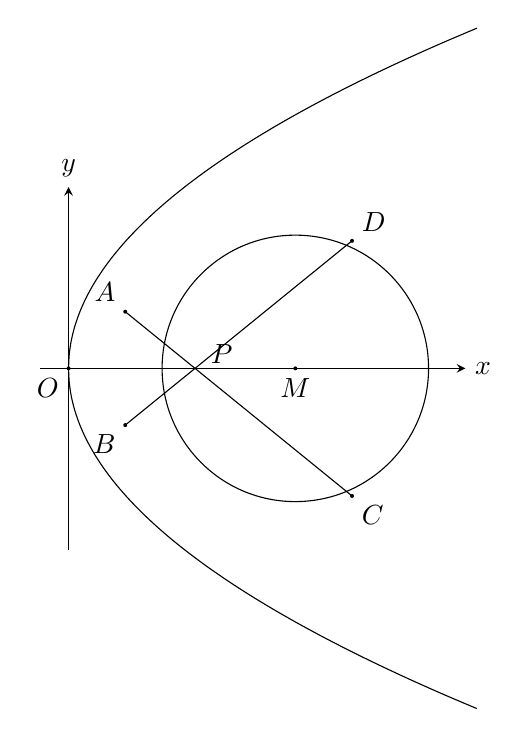
\begin{tikzpicture}[scale=.72,>=stealth]
\draw[->] (-.5,0)--(7,0) node[right] {$x$};
\draw[->] (0,-3.2)--(0,3.2) node[above] {$y$};
\draw[domain=0:6,smooth,variable=\x] plot ({\x*\x/5},{\x});
\draw[domain=0:6,smooth,variable=\x] plot ({\x*\x/5},{-\x});
\draw (4,0) circle (2.35);
\coordinate (A) at (1.0,1.0); \coordinate (B) at (1.0,-1.0);
\coordinate (C) at (5.0,-2.25); \coordinate (D) at (5.0,2.25);
\draw (A)--(C) (B)--(D);
\fill (0,0) circle (1pt) node[below left] {$O$};
\fill (4,0) circle (1pt) node[below] {$M$};
\fill (A) circle (1pt) node[above left] {$A$};
\fill (B) circle (1pt) node[below left] {$B$};
\fill (C) circle (1pt) node[below right] {$C$};
\fill (D) circle (1pt) node[above right] {$D$};
\node at (2.7,.25) {$P$};
\end{tikzpicture}
\end{center}
\nopagebreak[4]
（1） 求 $r$ 的取值范围；

（2） 当四边形 $ABCD$ 的面积最大时，求对角线 $AC\text{、}BD$ 的交点 $P$ 坐标。

\Needspace{4\baselineskip}
\textbf{解析}

\gksubpart{(1)}

\Needspace{5\baselineskip}
联立 $x=y^2$ 与圆方程，令 $t=y^2$，得

\nopagebreak[4]
\[
t^2-7t+16-r^2=0.
\]

四个不同交点要求两个不同的正根，故
\Needspace{5\baselineskip}
$4r^2-15>0$ 且 $16-r^2>0$，即

\nopagebreak[4]
\[
\frac{\sqrt{15}}2<r<4.
\]

\gksubpart{(2)}

设两根的平方根为 $u\text{、}v$，则 $u^2+v^2=7$。四边形面积为
\Needspace{5\baselineskip}
$S=(v^2-u^2)(u+v)$。令 $z=(u+v)^2$，则

\nopagebreak[4]
\[
S=z\sqrt{14-z},
\]

\Needspace{5\baselineskip}
其最大值在 $z=28/3$ 处取得。于是

\nopagebreak[4]
\[
uv=\frac{z-7}{2}=\frac76.
\]

由对称性，对角线交点的纵坐标为 $0$、横坐标为 $uv$，故
$P\left(\dfrac76,0\right)$。

\gkanswer{答案（1）：$\dfrac{\sqrt{15}}2<r<4$}

\gkanswer{答案（2）：$P\left(\dfrac76,0\right)$}

\end{answer}